\begin{figure}[ht!]
  \centering
  \caption{Graphical representation of data work} \label{fig:data_visualisation}
  \begin{subfigure}[b]{\textwidth}
  \centering
  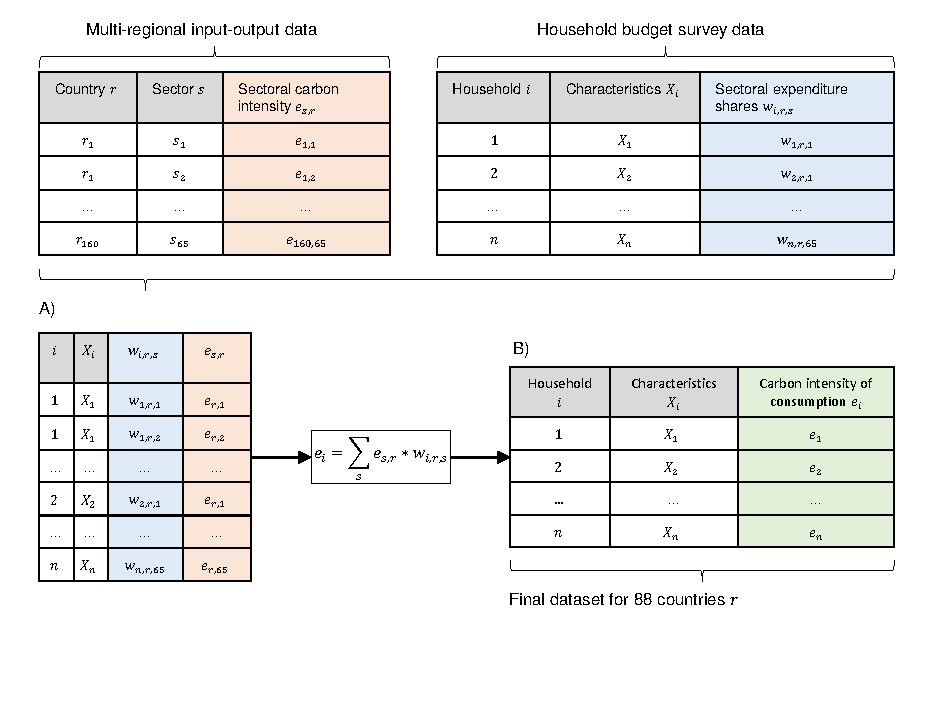
\includegraphics{1_Figures/Figures_Appendix/Graphical representation of data work_1.pdf}
  \caption{Combination of household-level data and multi-regional input-output data} \label{fig:data_visualisation_1}
  \begin{subcaption2}
    This figure shows the main properties of combining household-level data and multi-regional input-output data to calculate household-level carbon intensities of consumption $e_{i}$. Inputs are datasets with country-sector-level information about (direct and indirect) carbon intensities of output and datasets with household-level information about household characteristics and sectoral expenditure shares. Output is a dataset (B) with household-level information about household characteristics and carbon intensities of consumption $e_{i}$ for 88 countries.
  \end{subcaption2}
  \end{subfigure}
\end{figure}

\clearpage

\begin{figure}[ht!]\ContinuedFloat
   \begin{subfigure}[b]{\textwidth}
  \centering
  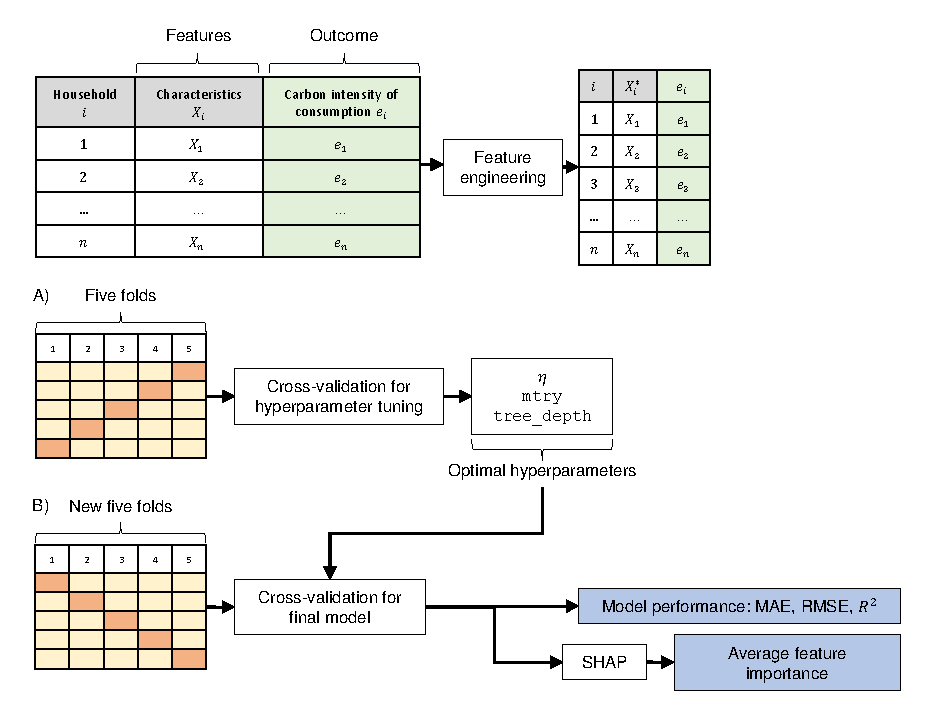
\includegraphics{1_Figures/Figures_Appendix/Graphical representation of data work_2.pdf}
  \caption{Feature engineering, hyperparameter tuning, and model evaluation} \label{fig:data_visualisation_2}
  \begin{subcaption2}
    This figure shows the main properties of feature engineering, hyperparameter tuning, and model evaluation. Input is a dataset with household-level information about household characteristics and carbon intensities of consumption $e_{i}$ for 88 countries. Household characteristics form a set of features. After feature engineering, we use fivefold cross-validation for hyperparameter tuning. Building on optimal hyperparameters, we use fivefold cross-validation for our final model. Output is a vector of model performance indicators (MAE, RMSE, R\textsuperscript{2}) and a measure of average feature importance for each country and feature, based on SHAP-values.
  \end{subcaption2}
\end{subfigure}
\end{figure}

\clearpage

\begin{figure}[ht!]\ContinuedFloat
   \begin{subfigure}[b]{\textwidth}
  \centering
  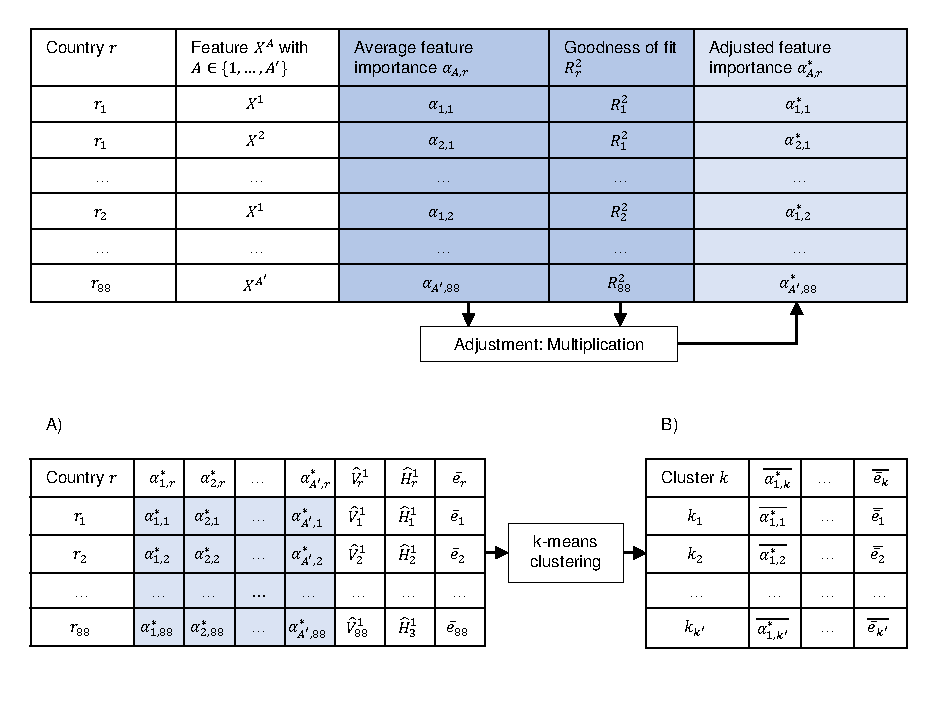
\includegraphics{1_Figures/Figures_Appendix/Graphical representation of data work_3.pdf}
  \caption{Identification of country clusters} \label{fig:data_visualisation_3}
  \begin{subcaption2}
    This figure shows the main properties of identifying country clusters. Input is a dataset with country-level information about average feature importance for each feature and models' goodness of fit (R\textsuperscript{2}). After adjusting feature importance, we use k-means clustering to identify a set of \textit{k'} clusters. We use average silhouette width for selection of the optimal number of clusters \textit{k'}. Output is a dataset with cluster-level information about average feature importance.
  \end{subcaption2}
\end{subfigure}
\end{figure}